\section{How Remy Produces a Congestion-Control Algorithm}
\label{s:design}

The above model may be viewed as a cooperative game that endpoints play. Given
packets to transmit (offered load) at an endpoint, the endpoint must
decide when to send packets in order to maximize its own objective
function. With a particular congestion-control algorithm running on
each endpoint, we can calculate each endpoint's expected score.

In the traditional game-theoretic framework, an endpoint's decision to
send or abstain can be evaluated after fixing the behavior of all
other endpoints. An endpoint makes a ``rational'' decision to send if
doing so would improve its expected score, compared with abstaining.

Unfortunately, when greater individual throughput is the desired
objective, on a best-effort packet-switched network like the Internet,
it is always advantageous to send a packet. In this setting, if every
endpoint acted rationally in its own self-interest, the resulting Nash
equilibrium would be congestion collapse!\footnote{Other researchers
  have grappled with this problem; for example, Akella et
  al.~\cite{Akella02} studied a restricted game, in which players are
  forced to obey the same particular flavor of TCP, but with the freedom
  to choose their additive-increase and multiplicative-decrease
  coefficients. Even with this constraint, the authors found that the Nash
  equilibrium is inefficient, unless the endpoints are restricted to
  run TCP Reno over a drop-tail buffer, in which case the equilibrium
  is unfair but not inefficient.}  This answer is unsatisfactory from
a protocol-design perspective, when endpoints have the freedom to send
packets when they choose, but the designer wishes to achieve an
efficient and equitable allocation of network capacity.

Instead, we believe the appropriate framework is that of {\em
  superrationality}~\cite{hofstadter1985metamagical}. Instead of
fixing the other endpoints' actions before deciding how to maximize
one endpoint's expected score, what is fixed is the common (but as-yet
unknown) algorithm run by all endpoints. As in traditional game
theory, the endpoint's goal remains maximizing its own self-interest,
but {\em with the knowledge} that other endpoints are reasoning the
same way and will therefore arrive at the same algorithm.

Remy's job is to find what that algorithm should
be.  We refer to a particular Remy-designed congestion-control
algorithm as a ``RemyCC,'' which we then implant into an existing
sender as part of TCP, DCCP~\cite{dccp}, congestion manager~\cite{cm},
or another module running congestion control.  The receiver is
unchanged (as of now; this may change in the future), but is expected
to send periodic ACK feedback.

Formally, we treat the problem of finding the best RemyCC under
uncertain network conditions as a search for the best policy for a
decentralized partially-observable Markov decision
process, or Dec-POMDP~\cite{Oliehoek2012}. This model originated from operations
research and artificial intelligence, in settings where independent
agents work cooperatively to achieve some goal. In the case of
end-to-end congestion control, endpoints are connected to a shared
network that evolves in Markovian fashion. At every time step, the
agents must choose between the actions of ``sending'' or
``abstaining,'' using observables from their receiver or from network
infrastructure.

\subsection{Compactly representing the sender's state}

In principle, for any given network, there is an {\em optimal}
congestion-control scheme that maximizes the expected total of the
endpoints' objective functions. Such an algorithm would relate (1) the
entire history of observations seen thus far (e.g.~the
contents and timing of every ACK) and (2) the entire history of
packets already sent, to the best action at any given moment between sending a new packet or abstaining. However, the search for such an algorithm is likely
intractable; on a general Dec-POMDP it is
NEXP-complete~\cite{Bernstein2002}.

Instead, we approximate the solution by greatly abridging the sender's
state. A RemyCC tracks just three state variables, which it updates
each time it receives a new acknowledgment:

\begin{enumerate}

\item An exponentially-weighted moving average (EWMA) of the
  interarrival time between new acknowledgments received ({\tt
    ack\_ewma}).

\item An exponentially-weighted moving average of the time between TCP
  sender timestamps reflected in those acknowledgments ({\tt
    send\_ewma}). A weight of $1/8$ is given to the new sample in both
  EWMAs.

\item The ratio between the most recent RTT and the minimum RTT seen
  during the current connection (\tt{rtt\_ratio}).

\end{enumerate}

Together, we call these three variables the {\em RemyCC memory}. It is
worth reflecting on these variables, which are the
``congestion signals'' used by any RemyCC. We narrowed the memory to
this set after examining and discarding quantities like the
most-recent RTT sample, the smoothed RTT estimate, and the difference
between the long-term EWMA and short-term EWMA of the observed packet
rate or RTT. In our experiments, adding extra state variables didn't improve
the performance of the resulting protocol, and each additional
dimension slows down the design procedure considerably. But we don't
claim that Remy's three state variables are the only set that works,
or that they are necessarily optimal for all situations a protocol
might encounter. We expect that any group of estimates that roughly
summarizes the recent history could form the basis of a workable
congestion-control scheme.

We note that a RemyCC's memory does not include the two
factors that traditional TCP congestion-control schemes use: packet
loss and RTT. This omission is intentional: a RemyCC that functions
well will see few congestive losses, because its objective function
will discourage building up queues (bloating buffers will decrease a
flow's score).  Moreover, avoiding packet loss as a congestion signal
allows the protocol to robustly handle stochastic (non-congestive)
packet losses without adversely reducing performance. We
avoid giving the sender access to the RTT (as opposed to the RTT
ratio), because we do not want it to learn different behaviors for
different RTTs.

 %The EWMA of the
%received rate and the sender timestamps in the ACKs is able to
%correctly assess the state of congestion along the network path.

At the start of each flow, before any ACKs have been received, the
memory starts in a well-known all-zeroes initial state. RemyCCs do not
keep state from one ``on'' period to the next, mimicking TCP's
behavior in beginning with slow start every time a new connection is
established (it is possible that caching congestion state is a good
idea on some paths, but we don't consider this here). Although RemyCCs
do not depend on loss as a congestion signal, they do inherit the
loss-recovery behavior of whatever TCP sender they are added to.

\subsection{RemyCC: Mapping the memory to an action}

A RemyCC is defined by how it maps values of the memory to output
\emph{actions}. Operationally, a RemyCC runs as a sequence of lookups
triggered by incoming ACKs. (The triggering by ACKs is
inspired by TCP's ACK clocking.)  Each time a RemyCC sender receives
an ACK, it updates its memory and then looks up the corresponding
action. It is Remy's job to pre-compute this lookup table during the design
phase, by finding the mapping that maximizes the expected value of the
objective function, with the expectation taken over the network model.

Currently, a Remy action has three components:

\begin{enumerate}

\item A multiple $m \geq 0$ to the current congestion window ({\tt cwnd}).

\item An increment $b$ to the congestion window ($b$ could be negative).

\item A lower bound $r > 0$ milliseconds on the time between
  successive sends.

\end{enumerate}

If the number of outstanding packets is greater than {\tt cwnd}, the
sender will transmit segments to close the window, but no faster than
one segment every $r$ milliseconds.

A RemyCC is defined by a set of piecewise-constant \emph{rules}, each one
mapping a three-dimensional rectangular region of the
three-dimensional memory space to a three-dimensional action:
$$
\langle {\tt ack\_ewma}, {\tt send\_ewma}, {\tt rtt\_ratio} \rangle \rightarrow
\langle m, b, r \rangle.
$$

\subsection{Remy's automated design procedure}

The design phase of Remy is an optimization procedure to efficiently
construct this state-to-action mapping, or \emph{rule table}.  Remy uses simulation of the senders on
various sample networks drawn from the network model, with
parameters drawn within the ranges of the supplied prior
assumptions. These parameters include the link rates, delays, the
number of sources, and the on-off distributions of the
sources. Offline, Remy
evaluates candidate algorithms on
millions of randomly generated network configurations. Because of the
high speed of current computers and the ``embarrassingly parallel''
nature of the task, Remy is able to generate congestion-control
algorithms within a few hours.

%For example, if one training
%network is the single-bottleneck (dumbbell) configuration (Figure
%\ref{fig:dumbbell}), four quantities provide the uncertainty: first,
%the maximum number of senders $n$ is unknown. Each sender turns ``on''
%and ``off'' according to some external process, e.g.~a heavy-tailed
%distribution of the byte length of each transmission, producing an
%uncertain number of senders currently ``on.''

\begin{figure}
\vspace{\baselineskip}
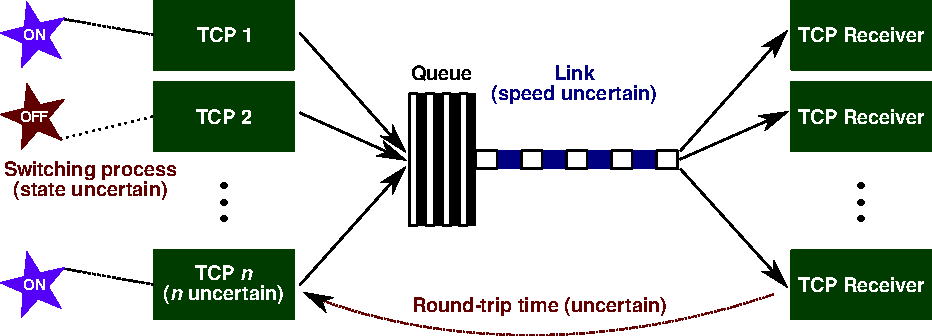
\includegraphics[width=\columnwidth]{dumbbell.pdf}
\caption{Dumbbell network with uncertainty.}
\label{fig:dumbbell}

\end{figure}

A single evaluation step, the innermost loop of Remy's design process,
consists of drawing 16 or more network specimens from the network
model, then simulating the RemyCC algorithm at each sender for 100
seconds on each network specimen. At the end of the simulation, the
objective function for each sender, given by Equation~\ref{eq:util},
is totaled to produce an overall figure of merit for the RemyCC. We
explore two cases, $\alpha = \beta = 1$ and $\alpha=2, \delta =
0$. The first case corresponds to proportional throughput and delay
fairness, maximizing $$U = \log (\mbox{throughput}) - \delta \cdot
\log (\mbox{delay}),$$ with $\delta$ specifying the importance placed
on delay vs.~throughput. The second case corresponds to minimizing the
potential delay of a fixed-length transfer, by maximizing $$U =
-\frac{1}{\mbox{throughput}}.$$

%\subsection{The optimization procedure}

Remy initializes a RemyCC with only a single rule. Any values of the
three state variables (between 0 and 16,384) are mapped to a default
action where $m = 1$, $b = 1$, $r = 0.01$.

Each entry in the rule table has an ``epoch.''
Remy maintains a global epoch number, initialized to 0. Remy's search
for the ``best'' RemyCC given a network model is a series of greedy
steps to build and improve the rule table:

\begin{enumerate}

\item\textbf{Set all rules to the current epoch.} 

\item \textbf{Find the most-used rule in this epoch.} Simulate the
  current RemyCC and see which rule in the current epoch
  receives the most use.  If no such rules were used, go
  to step 4.

\item \textbf{Improve that action until we can't anymore.} Focus on
  this rule and find the best action for it. Draw at least 16 network
  specimens from the model, and then evaluate roughly 100 candidate
  increments to the current action, increasing geometrically in
  granularity as they get further from the current value. For example,
  evaluate $r \pm 0.01$, $r \pm 0.08$, $r \pm 0.64$, \ldots, taking
  the Cartesian product with the alternatives for $m$ and $b$.

  The modified action is evaluated by substituting it \emph{into all
    senders} and repeating the simulation in parallel. We use the same
  random seed and the same set of specimen networks in the simulation of
  each candidate action to reduce the effects of random variation.

  If any of the candidates is an improvement, replace the action with
  the best new action and repeat the search, still with the same
  specimen networks and random seed. Otherwise, increment the epoch
  number of the current rule and go back to step~2.

\item \textbf{If we run out of rules in this epoch.} Increment the
  global epoch. If the new epoch is a multiple of a parameter, $K$,
  continue to step 5. Otherwise go back to step 1. We use $K = 4$ to
  balance structural improvements vs.~honing the existing structure.

\item \textbf{Subdivide the most-used rule.} Recall that each rule
  represents a mapping from a three-dimensional rectangular region of
  memory space to a single action. In this step, find the most-used
  rule, and the median memory value that triggers it. Split the rule
  at this point, producing eight new rules (one per dimension of the
  memory-space), each with the same action as before. Then return to
  step 1.

\end{enumerate}

By repeating this procedure, the structure of a RemyCC's rule table
becomes an
octree~\cite{octree}
of memory regions. Areas of the memory space more likely to occur
receive correspondingly more attention from the optimizer, and are
subdivided into smaller bins that yield a more granular function
relating memory to action. \emph{Which} rules are more often triggered
depends on every endpoint's behavior as well as the network's
parameters, so the task of finding the right structure for the rule
table is best run alongside the process of optimizing existing rules.

To the best of our knowledge, this dynamic partitioning approach is
novel in the context of multi-agent optimization. The ``greedy''
approach in step 2 is key to the computational tractability and
efficiency of the search because it allows us to prune the search
space. Dividing the memory space into cells of different size
proportional to their activity produces a rule table
whose granularity is finer in regions of higher use. An improvement to
consider in the future is to divide a cell only if the actions at its
boundaries markedly disagree.\footnote{We thank Leslie Kaelbling for
  this suggestion.}
